\section{Sformułowanie problemu}
\label{sec:sformulowanie-problemu}
W tym rozdziale opisany jest Internet Rzeczy pod względem problemów badawczego i projektowego, jakie zostały w pracy rozwiązane. Zaprezentowane są tutaj podejścia, jakie zdecydowałem się zastosować w moim projekcie, oraz wyjaśnienie dlaczego są to rozwiązania lepsze od innych. 

\subsection{Struktura IoT}
Internet Rzeczy należy rozumieć jako system, w którym przedmioty mogą komunikować się między sobą, za pośrednictwem człowieka lub bez jego udziału.
Dobrym schematem obrazującym tą koncepcję jest \autoref{fig:iot_base}. Widać tutaj wyraźnie, że to podejście jest uniwersalne. Z rysunku wynika, że istnieje podział na cztery główne części.

\begin{figure}[!htbp]
	\centering
	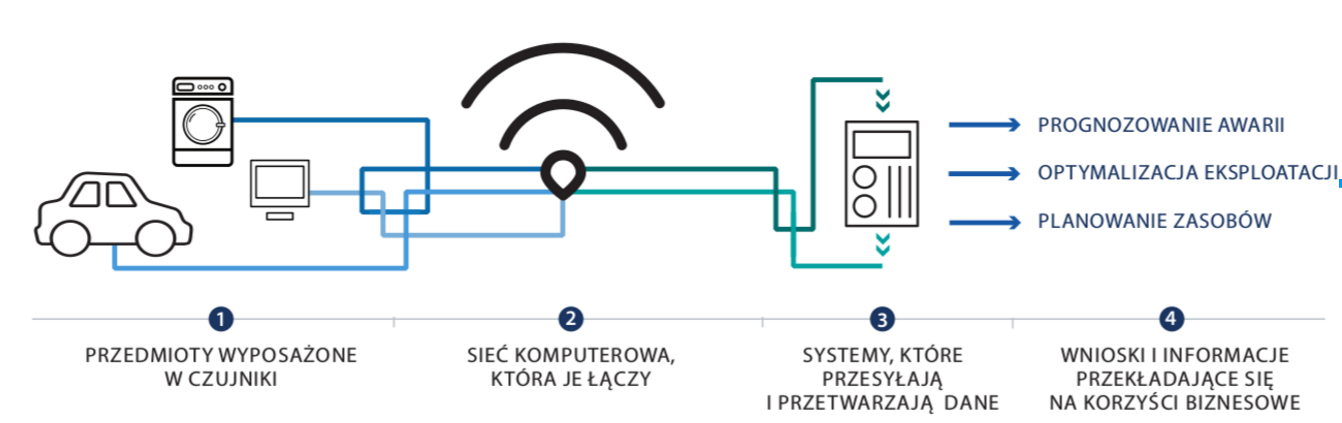
\includegraphics[width=1.0\textwidth]{images/iot.png}
	\caption[Idea funkcjonowania rozwiązań Internetu Rzeczy.]{Idea funkcjonowania rozwiązań Internetu Rzeczy}
	\label{fig:iot_base}
\end{figure}

\subsubsection{Przedmioty wyposażone w czujniki}
Naszą sieć IoT możemy zbudować praktycznie w każdej dziedzinie. ża pomocą jednego systemu mamy możliwość sterowania każdym rodzajem urządzeń - od sprzętów AGD/RTV po samochody, czy domy. Strefy zastosowań urządzeń IoT przedstawia \autoref{fig:zastosowania_iot}. Widać wyraźnie, że istnieją one wszędzie, potwierdzeniem tego faktu jest \autoref{fig:ile_urzadzen} opisany szerzej w \autoref{sec:benefits_conclusions}.

\begin{figure}[!htbp]
	\centering
	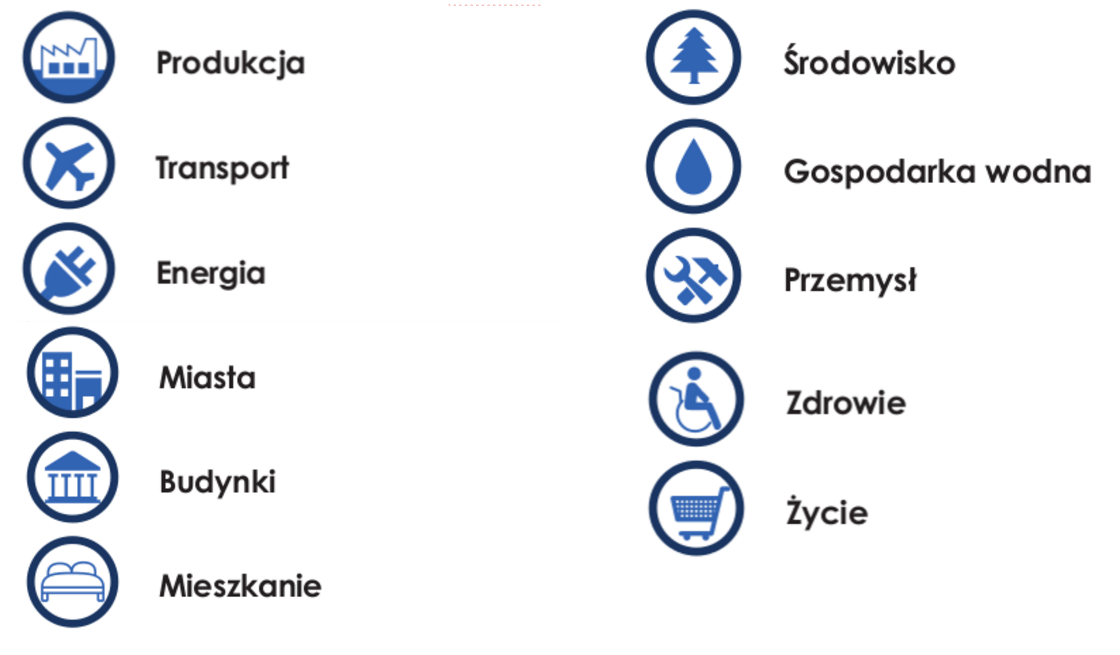
\includegraphics[width=1.0\textwidth]{images/zastosowania.png}
	\caption[Obszar zastosowania IoT.]{Obszar zastosowania IoT}
	\label{fig:zastosowania_iot}
\end{figure}
\subsubsection{Sieć komputerowa, która je łączy}
Tutaj mamy pole do popisu, bo tak naprawdę istnieje bardzo wiele interfejsów pozwalających na łączenie urządzeń w jedną integralną całość. Do wyboru mamy - od tych bardziej znanych standardów m.in:

\begin{itemize}
	\item Wi-Fi
	\item Bluetooth
\end{itemize}
Po te mniej znane, jednak równie często wykorzystywane:
\begin{itemize}
	\item NFC 
	\item Z-Wave 
\end{itemize}
Istotne jest połączenie takich urządzeń z Internetem, ponieważ w innym wypadku nie będzie możliwości sterowania tymi urządzeniami z zewnątrz. Wymaga to jednak dodatkowej infrastruktury, więcej na ten temat w TODO.

\subsubsection{Systemy, które przetwarzają i przesyłają dane}
Posiadając już podpięte urządzenia do sieci, musimy jeszcze mieć czym nimi sterować/przetwarzać dane itp. Mamy możliwość instalacji urządzeń tych bardziej profesjonalnych, dedykowanych dla konkretnego klienta, jak np. \autoref{fig:panel_ogrzewanie}. Jest to panel do sterowania ogrzewaniem w domu firmy proav. Poprzez te bardziej uniwersalne, jak chociażby smartphone z systemem android/ios/windows.

\begin{figure}[!htbp]
	\centering
	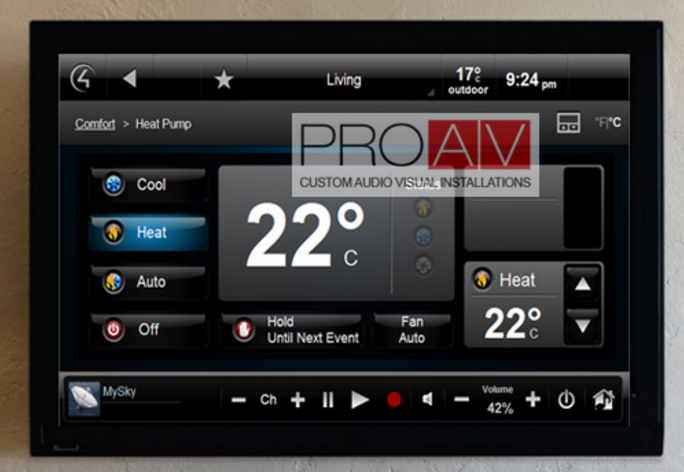
\includegraphics[width=0.7\textwidth]{images/panel_ogrzewanie.png}
	\caption[Panel do sterowania ogrzewaniem.]{Panel do sterowania ogrzewaniem}
	\label{fig:panel_ogrzewanie}
\end{figure}

\subsubsection{Wnioski i informacje przekładające się na korzyści biznesowe}
\label{sec:benefits_conclusions}
Innym zobrazowaniem idei Internetu Rzeczy jest \autoref{fig:iot_short}.
\begin{figure}[!htbp]
	\centering
	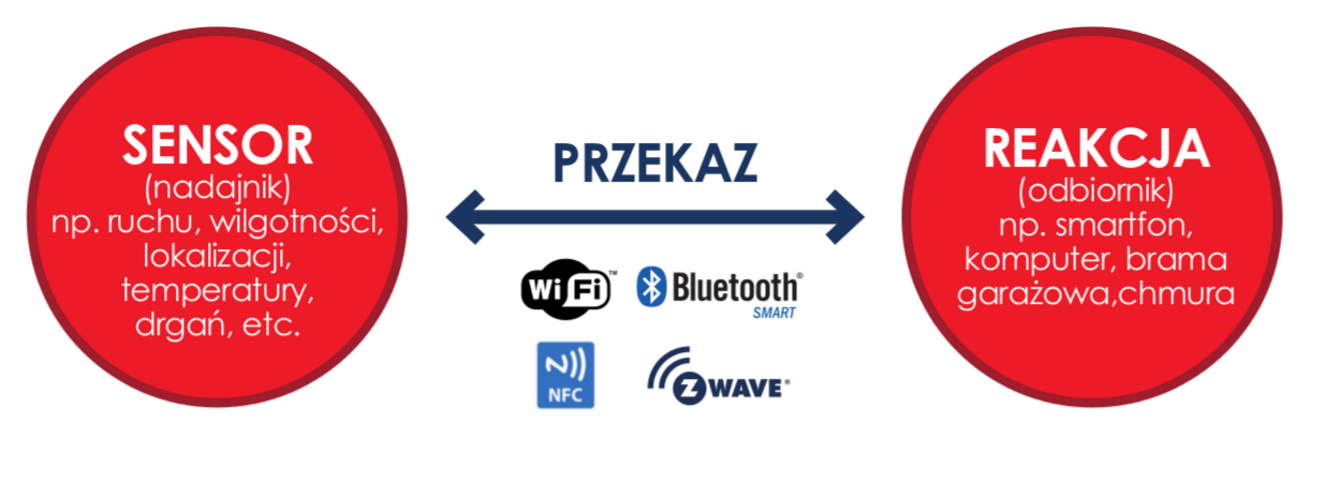
\includegraphics[width=1.0\textwidth]{images/iot_short.png}
	\caption[System wymiany informacji.]{System wymiany informacji}
	\label{fig:iot_short}
\end{figure}
Widać tutaj wszystko to co zostało pokrótce przedstawione w tym rozdziale. 
Ważnym wyznacznikiem, który przekonał mnie do napisania tej pracy był fakt, że liczba urządzeń IoT drastycznie wzrasta w czasie. Przedstawia to \autoref{fig:ile_urzadzen}, przewidywania są takie, że ich liczba do 2020 wzrośnie do 25 bilionów i już dawno przekroczyła liczbę ludności na świecie. 

\begin{figure}[!htbp]
	\centering
	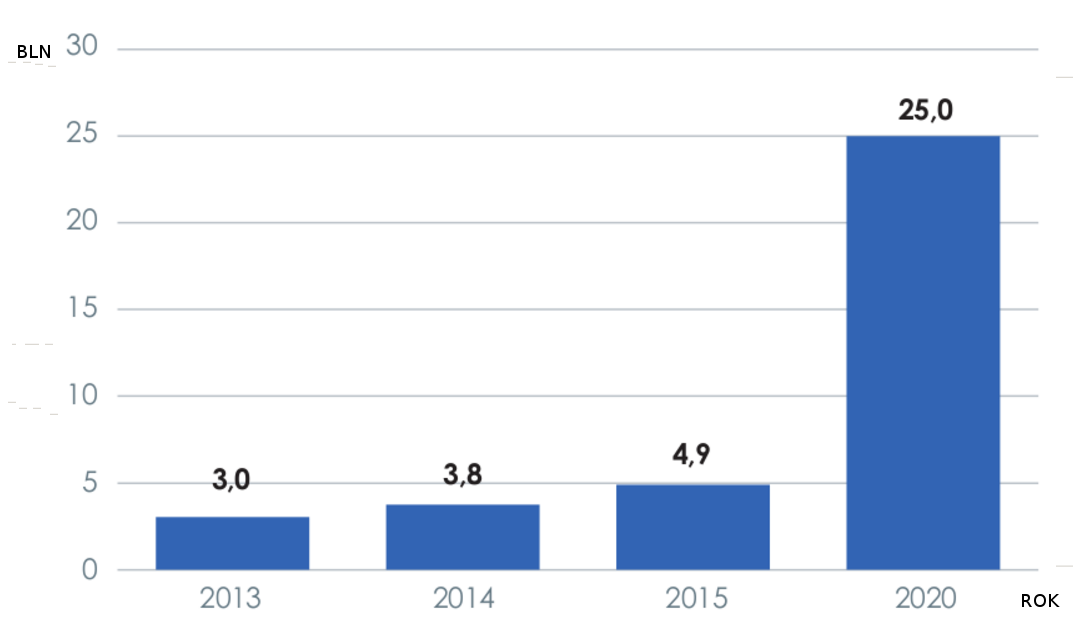
\includegraphics[width=1.0\textwidth]{images/ile_urzadzen.png}
	\caption[Liczba urządzeń Internetu Rzeczy.]{Liczba urządzeń Internetu Rzeczy}
	\label{fig:ile_urzadzen}
\end{figure}

Dobrym wyznacznikiem zmian czekających nas w najbliższym czasie jest \autoref{fig:internet_share}. Możemy zaobserwować wyraźny spadek wykorzystania zasobów Internetowych przez zwykłe komputery w ciągu kolejnych kilku lat. Już tym momencie stanowi on mniejszość spośród wykorzystania wszystkich zasobów w gospodarstwie domowym. Widać natomiast stopniowy wzrost użycia Internetu przez inne urządzenia. Wynika to z faktu posiadania przez każdego człowieka coraz to więcej urządzeń mobilnych i chęci zautomatyzowania kolejnych aspektów życia codziennego. 
\begin{figure}[!htbp]
	\centering
	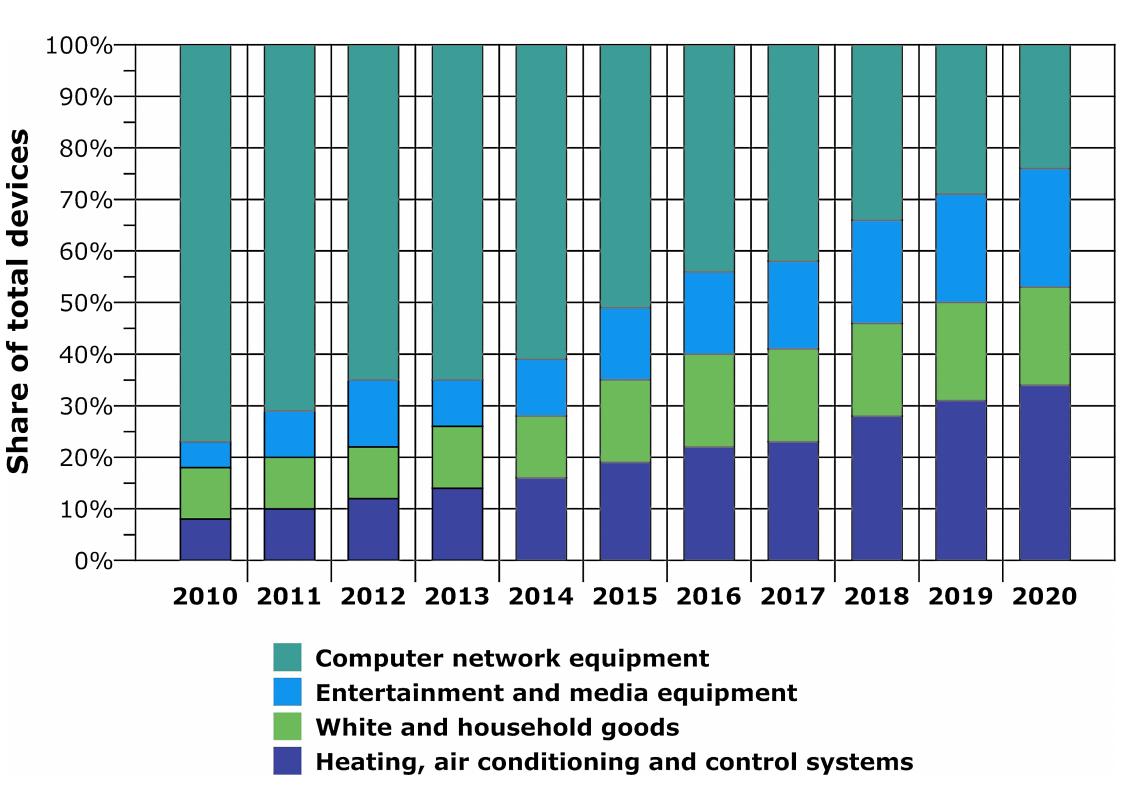
\includegraphics[width=1.0\textwidth]{images/internet_share.png}
	\caption[Udział poszczególnych urządzeń w wykorzystaniu zasobów Internetu w gospodarstwie domowym.]{Udział poszczególnych urządzeń w wykorzystaniu zasobów Internetu w gospodarstwie domowym}
	\label{fig:internet_share}
\end{figure}


\subsection{Rozwój i bariery}
Istnieją pewne aspekty, które są wyznacznikiem rozwoju systemu działającego pod szyldem Internetu Rzeczy. Proces miniaturyzacji jest jednym z nich, dzięki niemu możliwe jest korzystanie z mikrokontrolerów praktycznie w każdym urządzeniu. Ważnym elementem jest tutaj również rozwój technologii mobilnych i bezprzewodowego dostępu do Internetu. Te dwa główne aspekty powodują szybki rozwój IoT, jednak istnieją takie, które go hamują. Wciąż dużym ograniczeniem jest zasilanie. Baterie są coraz bardziej żywotne, jednak mają swoją wadę - trzeba je ładować. Często jest to duże ograniczenie, biorąc pod uwagę liczbę tych urządzeń działających samodzielnie. Innym ograniczeniem może okazać się protokół IPv4 (ok 4 mld urządzeń), dlatego często trzeba używać infrastruktury, która zapewni nam prywatne adresy IP. 

Istotnym wyzwaniem jest wytworzenie jednolitych standardów dotyczących bezpieczeństwa danych i poufności. Nie chcemy doprowadzić do sytuacji, w której dostęp do inteligentnego domu dostanie nieuprawniona osoba. 

\subsection{Dobór urządzenia}
Na samym początku pojawiło się pytanie jakiego rodzaju urządzenia powinienem użyć. Pytanie to jest zasadnicze, dlatego poświęciłem dużo czasu na zgłębienie tego tematu. Przeglądając różnego rodzaju interfejsy, te bardziej uniwersalne jak i te podstawowe, doszedłem do wniosku, że warto poświęcić więcej czasu na stworzenie czegoś od nowa i nauczenie się jak takie urządzenia działają od środka. Decyzja ta była o tyle trudna, że nie byłem pewien jaki będzie miała skutek dla całej pracy. Płytkę PCB wydrukowałem ręcznie i powstały dwa prototypy tego urządzenia (więcej na ten temat w \autoref{sec:hardware}). Samo urządzenie przedstawia \autoref{fig:device}
\begin{figure}[!htbp]
	\centering
	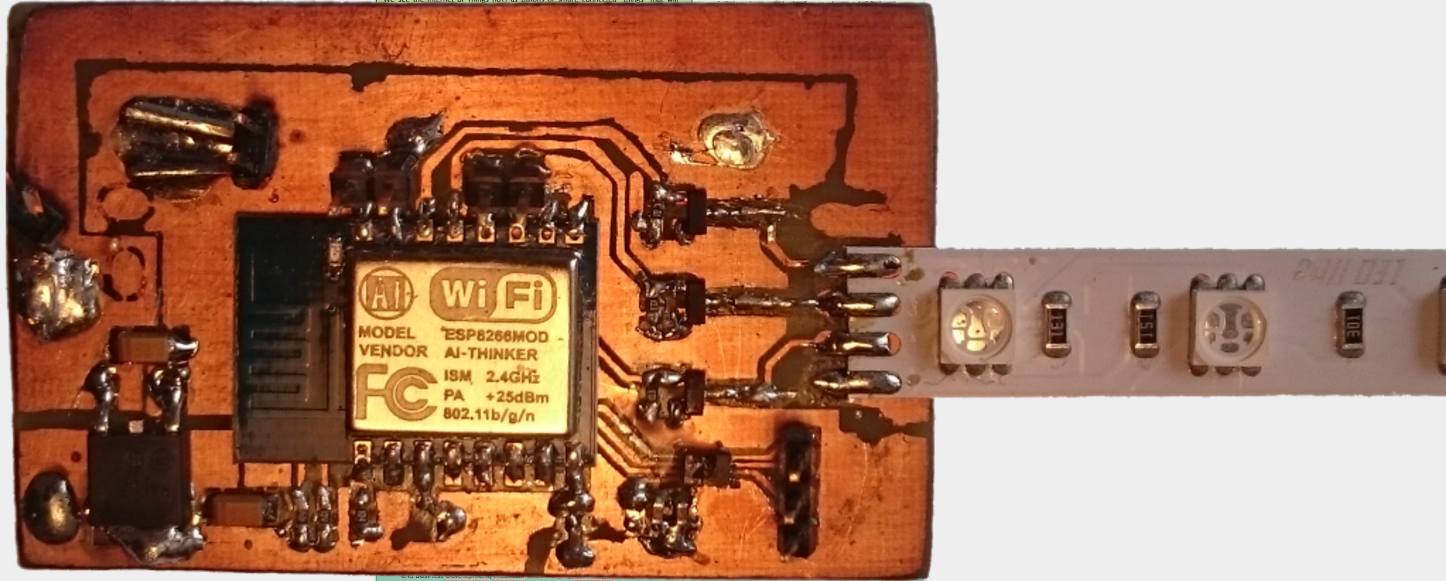
\includegraphics[width=1.0\textwidth]{images/device.png}
	\caption[Urządzenie PCB.]{Urządzenie PCB}
	\label{fig:device}
\end{figure}

\subsection{Analiza zagrożeń}
Wykonalność projektu jest obarczona pewnym ryzykiem. Jest ono głównie związane z możliwą nieznajomością obranych w późniejszym czasie technologii oraz małym doświadczeniem w dziedzinie Internetu rzeczy.

Kolejnym zagrożeniem jest ograniczony czas. Proponowane rozwiązanie zakłada stworzenie prototypu urządzenia, a następnie aplikacji, więc stworzenie układu będzie konieczne do uruchomienia i przetestowania całości.
